\section{Auswertung}
\label{sec:Auswertung}Jegliche Fehlerrechnung wurde mit der python-Bibliothek uncertainties \cite{uncertainties} absolviert.
Trotz dessen sind die Formeln für die Unsicherheiten in den jeweiligen Abschnitten angegeben.
Allgemeine Rechnungen wurden mit der python-Bibliothek numpy \cite{numpy} automatisiert.  
Die graphischen Unterstützungen wurden mit Hilfe der python-Bibliothek matplotlib \cite{matplotlib}
\subsection{Verifizierung der Funktion eines phasenempfindlichen Gleichrichters}
\label{sec:phase}
\begin{figure}
    \begin{subfigure}{0.48 \textwidth}
        \centering
        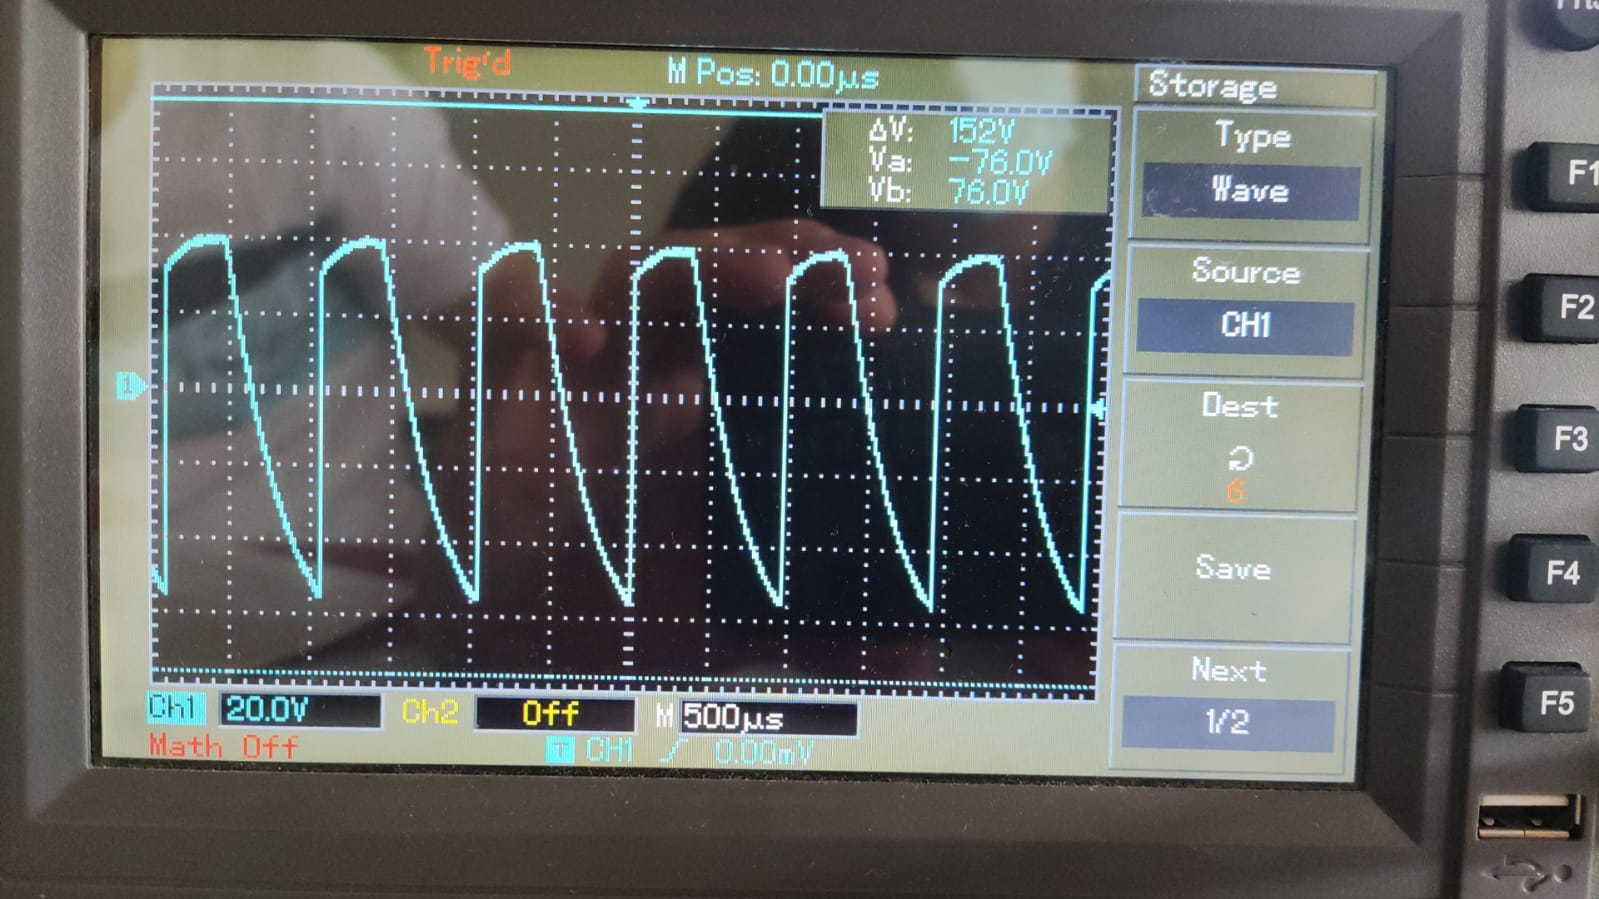
\includegraphics[height = 3.5cm]{data_scripts/pics/0o.jpeg}
        \caption{Ohne Rauschen}
    \end{subfigure}
    \hfill
    \begin{subfigure}{0.48 \textwidth}
            \centering
            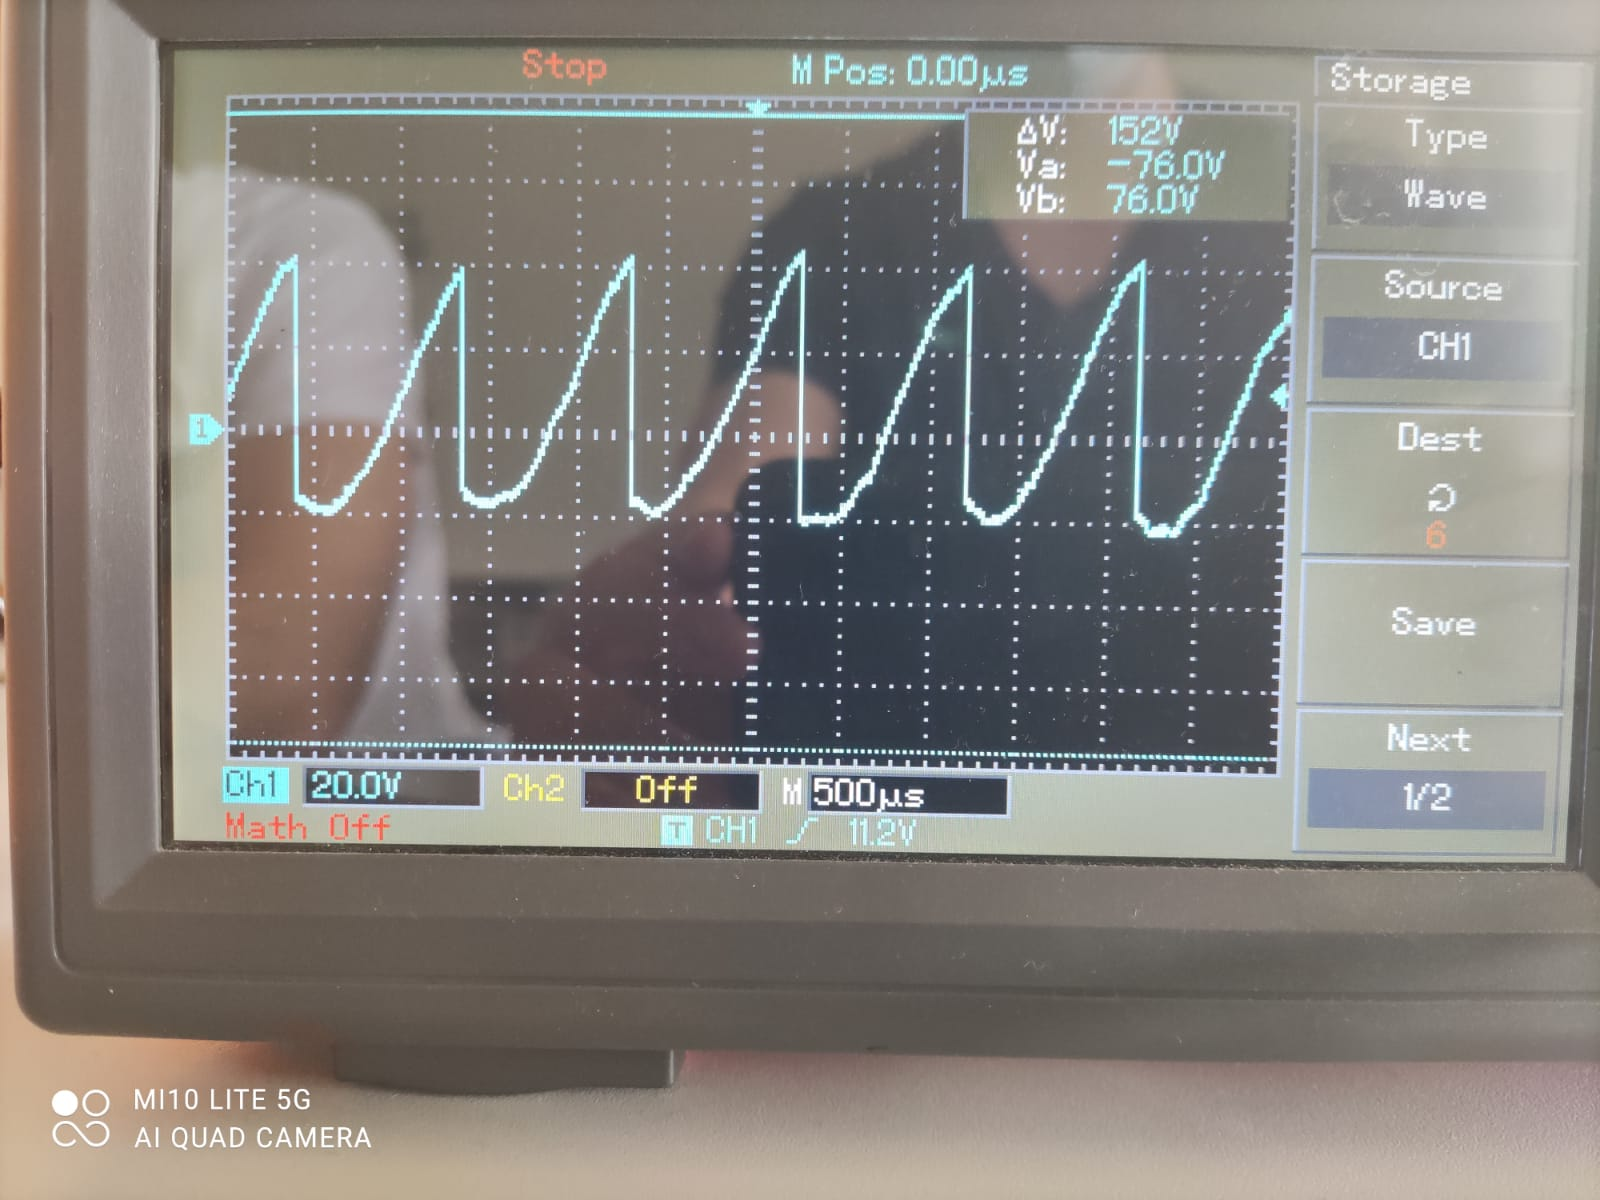
\includegraphics[height = 3.5cm]{data_scripts/pics/0m.jpeg}
            \caption{Mit Rauschen}
    \end{subfigure}
    \caption{Ausgangsspannung bei $\phi = \ang{0;;}$}
\end{figure}
\begin{figure}
    \begin{subfigure}{0.48 \textwidth}
        \centering
        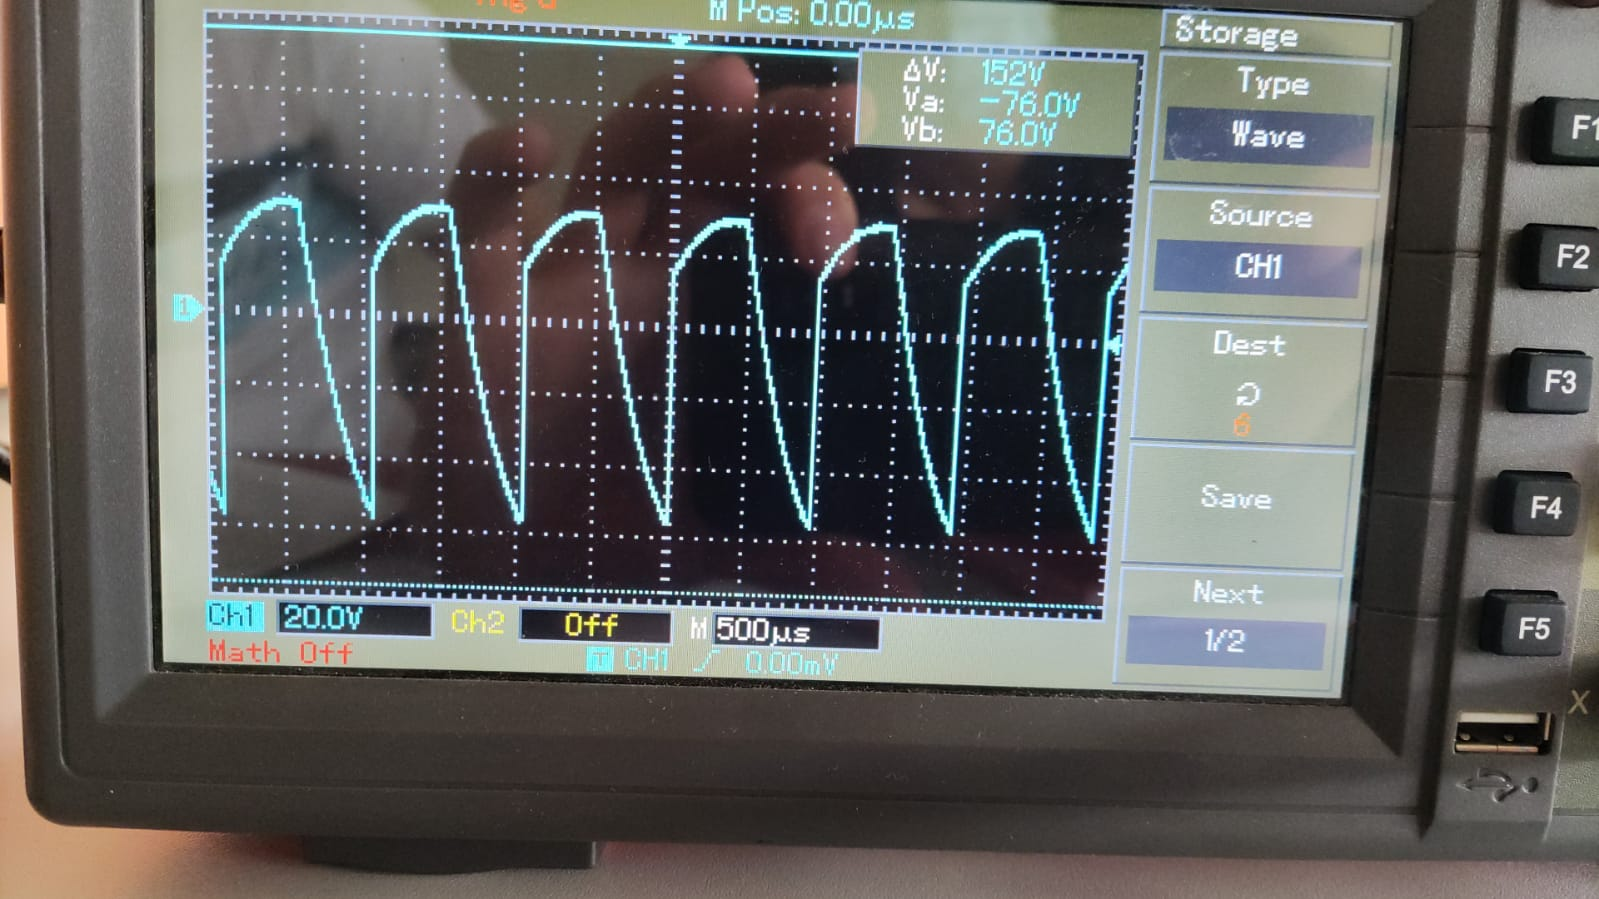
\includegraphics[height = 3.5cm]{data_scripts/pics/30o.jpeg}
        \caption{Ohne Rauschen}
    \end{subfigure}
    \hfill
    \begin{subfigure}{0.48 \textwidth}
            \centering
            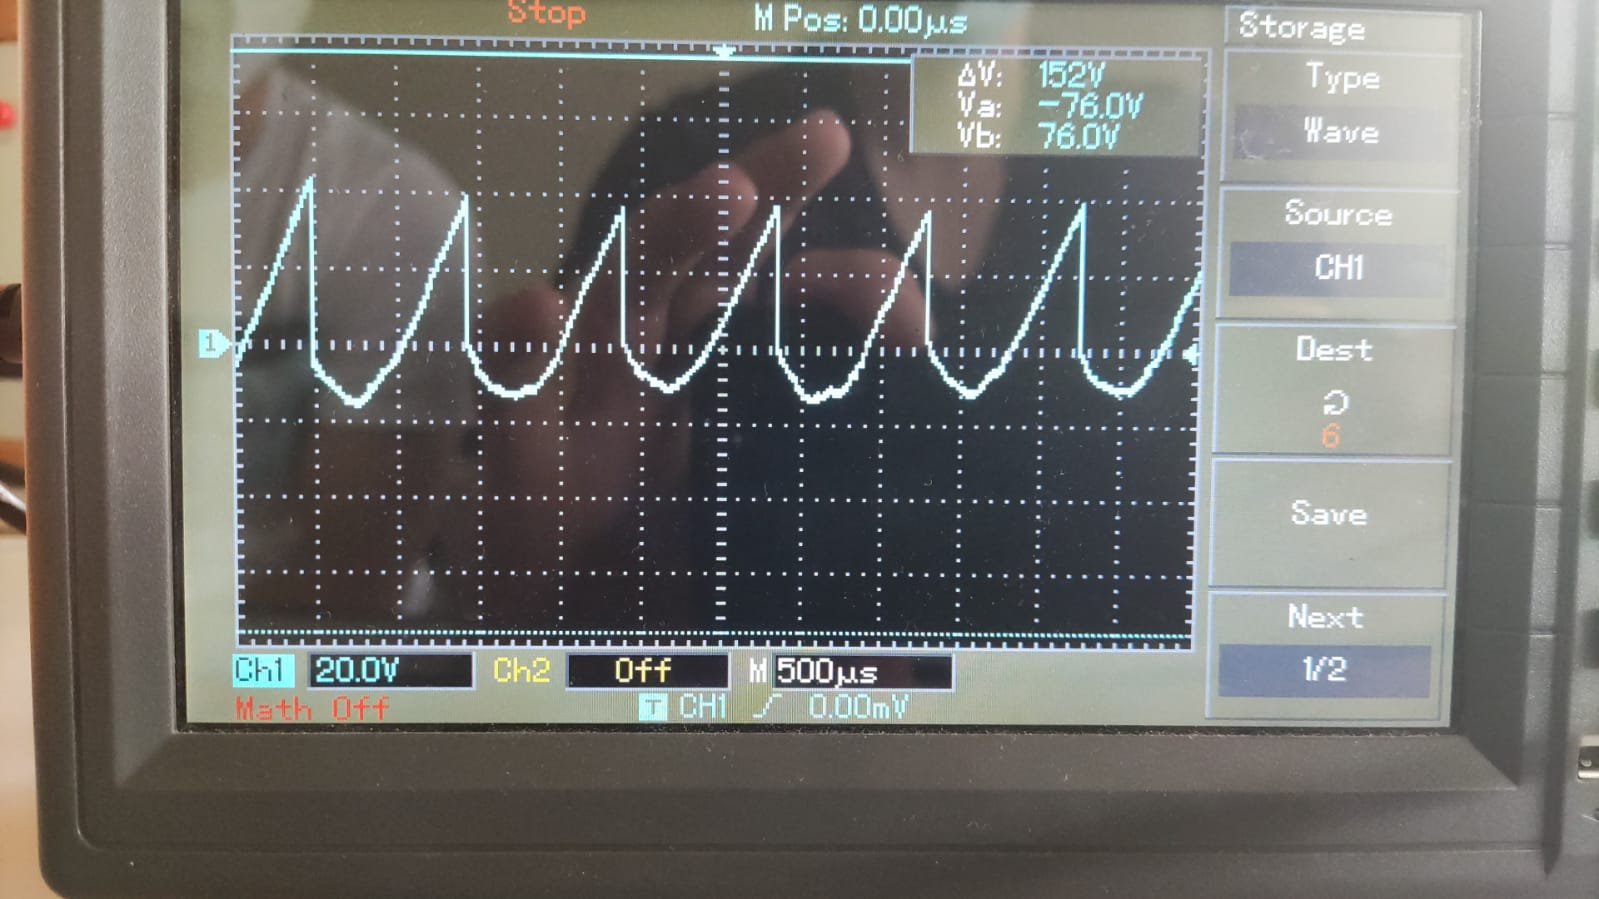
\includegraphics[height = 3.5cm]{data_scripts/pics/30m.jpeg}
            \caption{Mit Rauschen}
    \end{subfigure}
    \caption{Ausgangsspannung bei $\phi = \ang{30;;}$}
\end{figure}
\begin{figure}
    \begin{subfigure}{0.48 \textwidth}
        \centering
        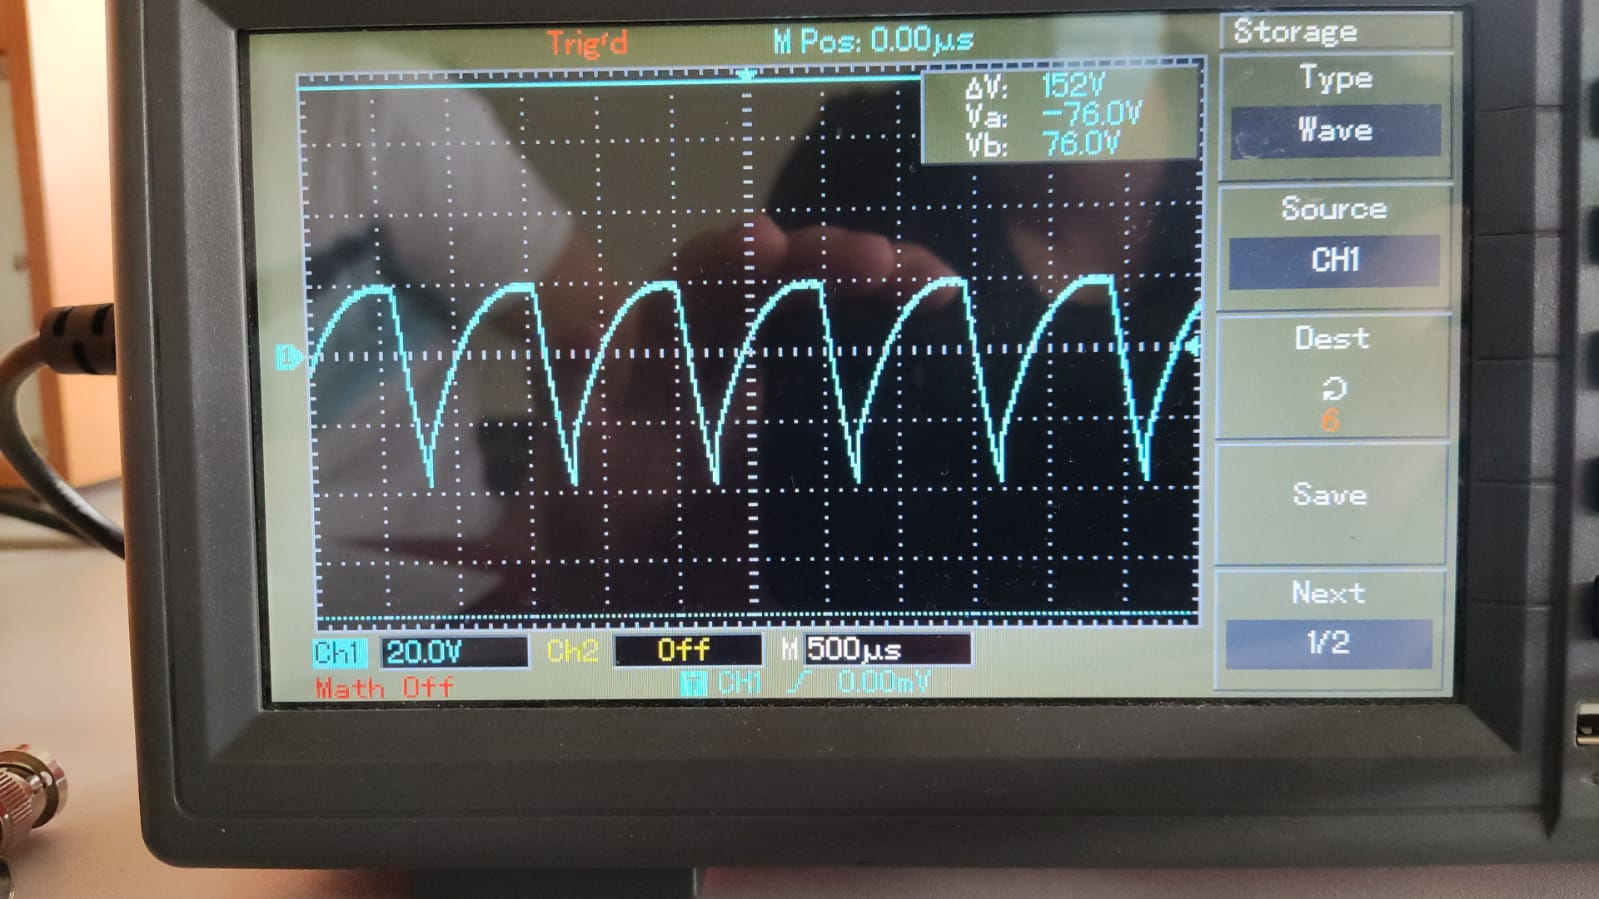
\includegraphics[height = 3.5cm]{data_scripts/pics/60o.jpeg}
        \caption{Ohne Rauschen}
    \end{subfigure}
    \hfill
    \begin{subfigure}{0.48 \textwidth}
            \centering
            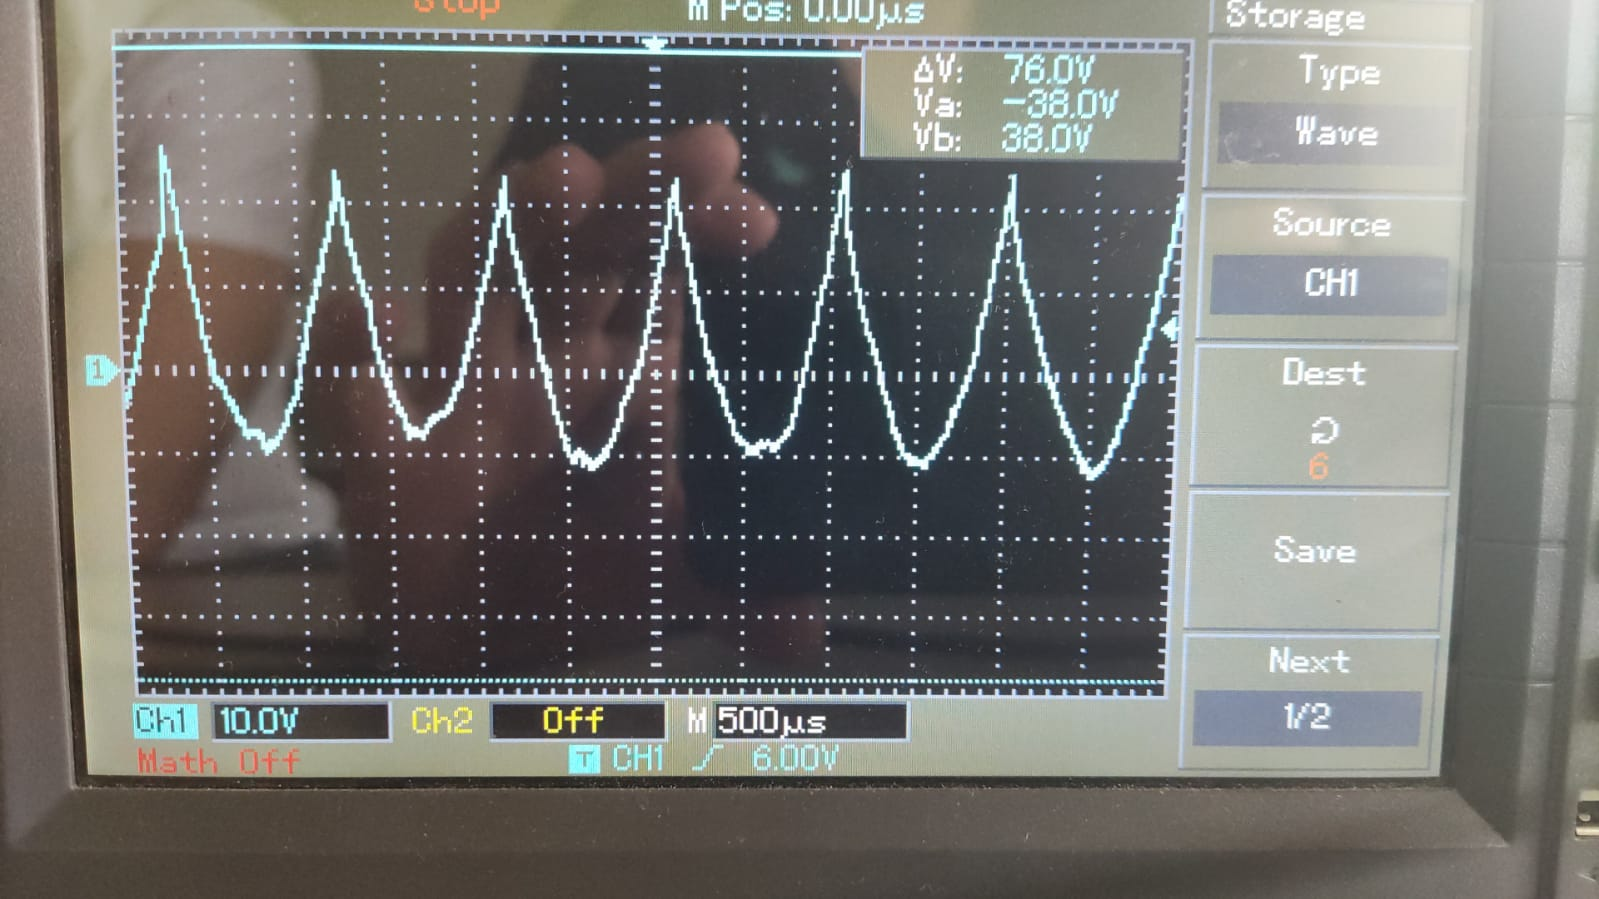
\includegraphics[height = 3.5cm]{data_scripts/pics/60m.jpeg}
            \caption{Mit Rauschen}
    \end{subfigure}
    \caption{Ausgangsspannung bei $\phi = \ang{60;;}$}
\end{figure}
\begin{figure}
    \begin{subfigure}{0.48 \textwidth}
        \centering
        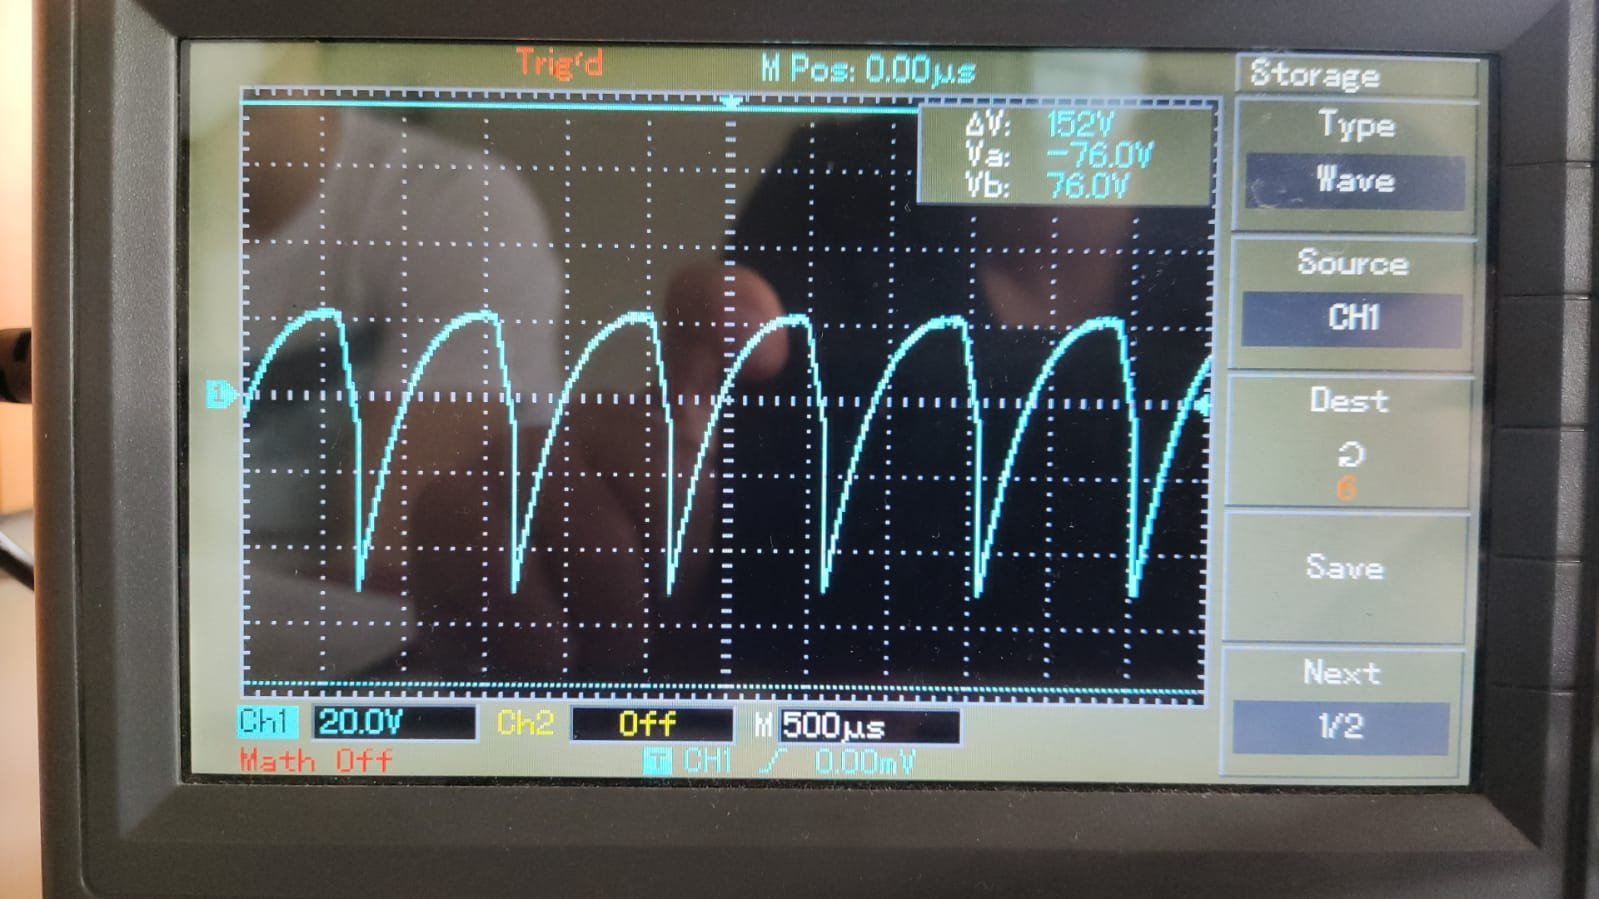
\includegraphics[height = 3.5cm]{data_scripts/pics/90o.jpeg}
        \caption{Ohne Rauschen}
    \end{subfigure}
    \hfill
    \begin{subfigure}{0.48 \textwidth}
            \centering
            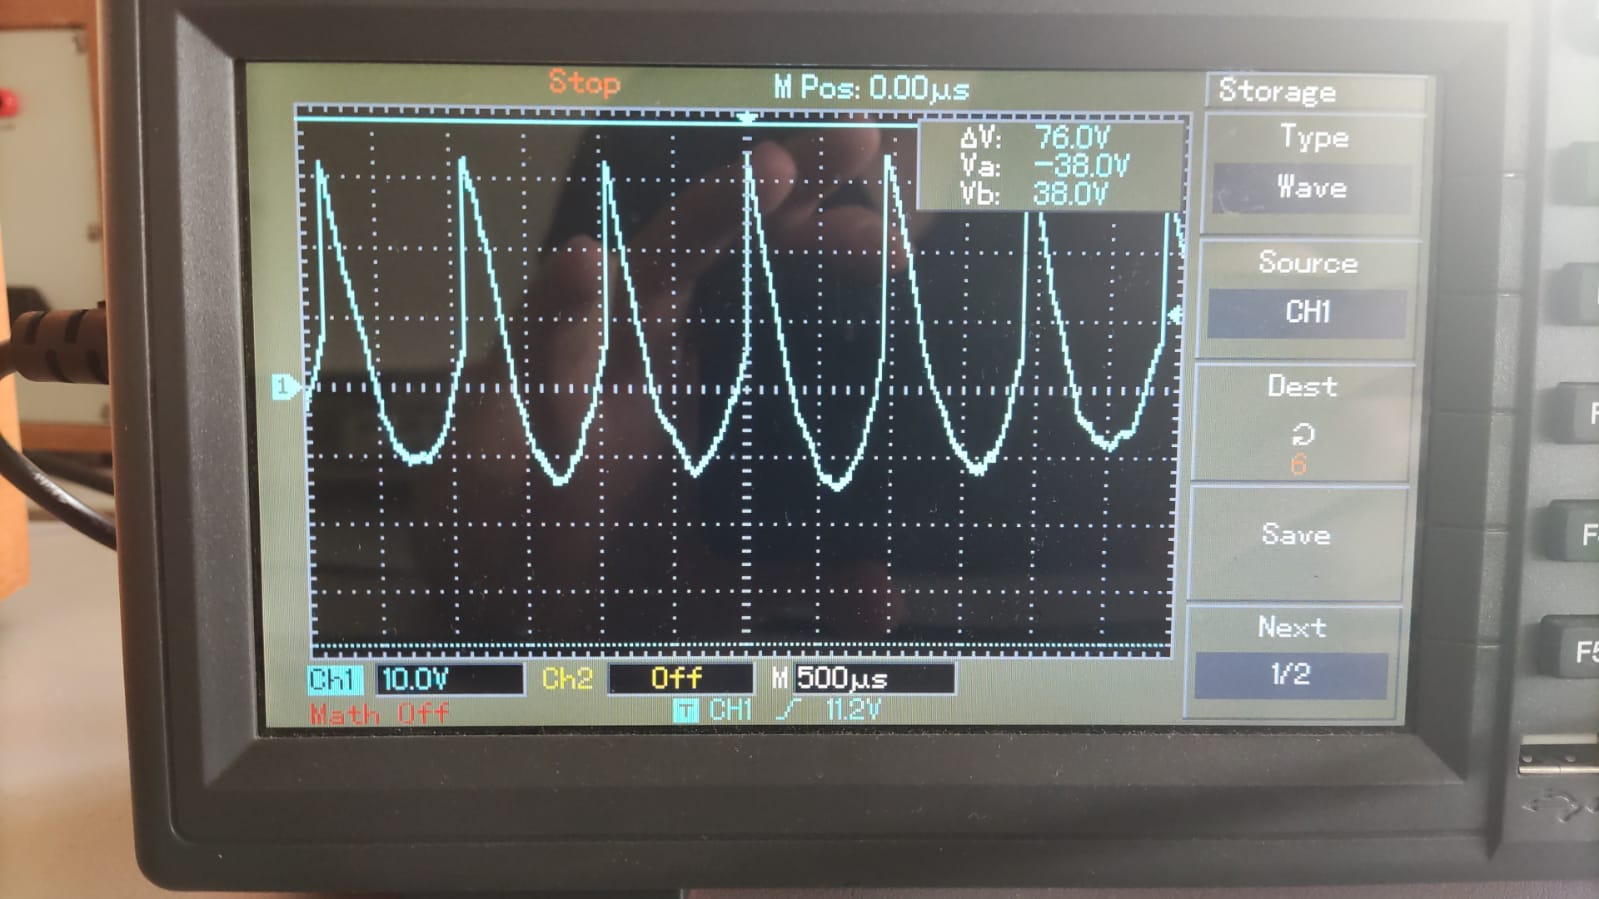
\includegraphics[height = 3.5cm]{data_scripts/pics/90m.jpeg}
            \caption{Mit Rauschen}
    \end{subfigure}
    \caption{Ausgangsspannung bei $\phi = \ang{90;;}$}
\end{figure}
\begin{figure}
    \begin{subfigure}{0.48 \textwidth}
        \centering
        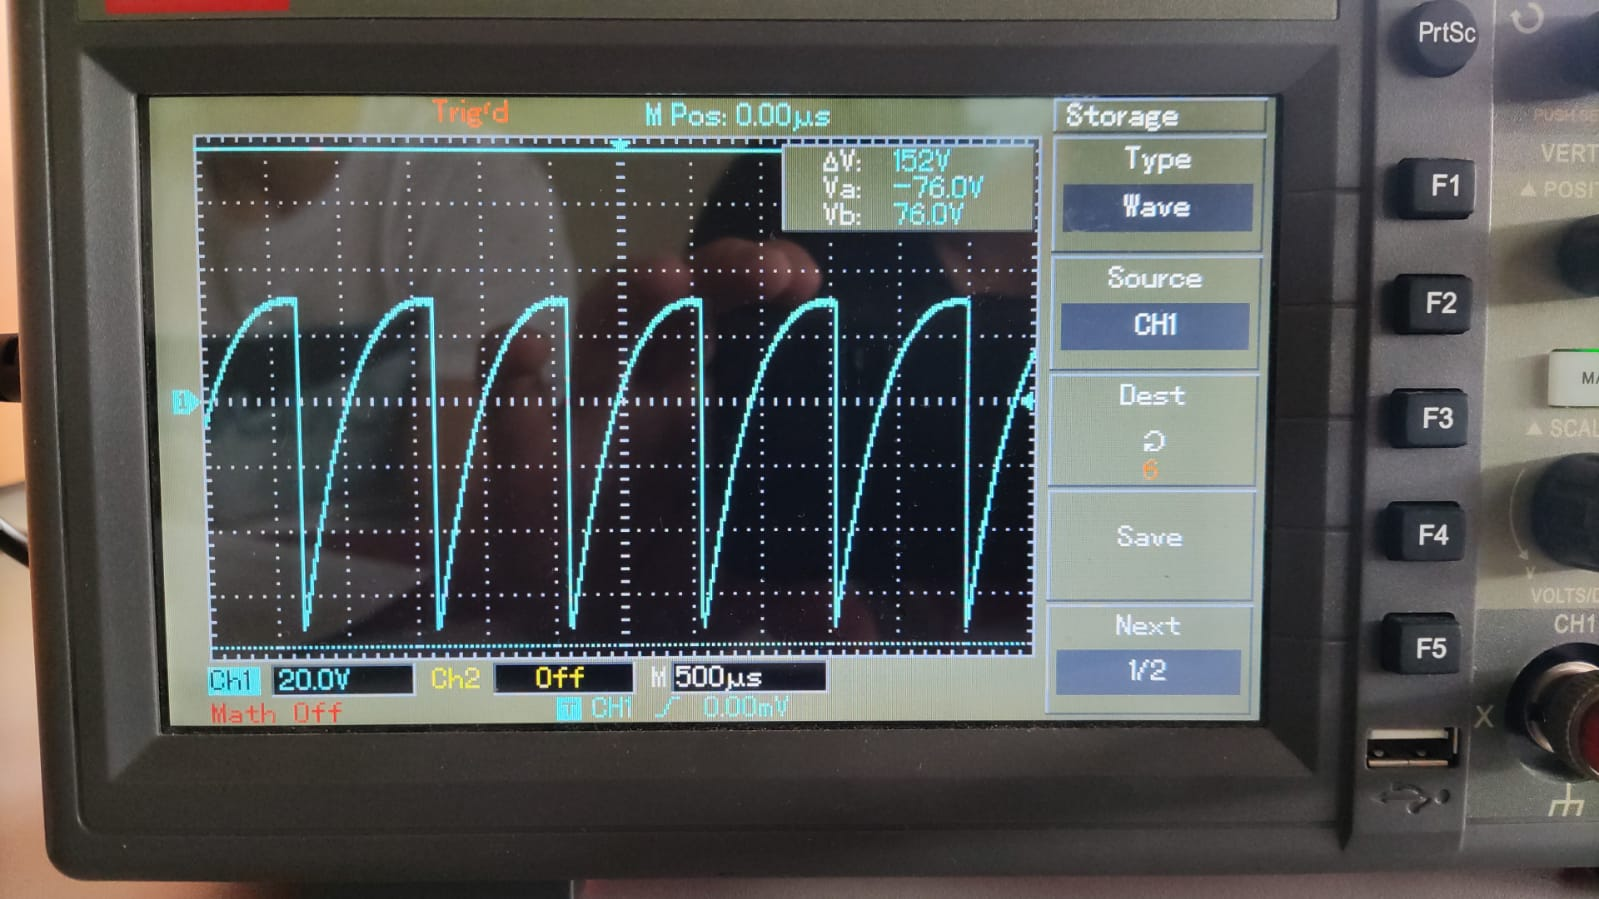
\includegraphics[height = 3.5cm]{data_scripts/pics/120o.jpeg}
        \caption{Ohne Rauschen}
    \end{subfigure}
    \hfill
    \begin{subfigure}{0.48 \textwidth}
            \centering
            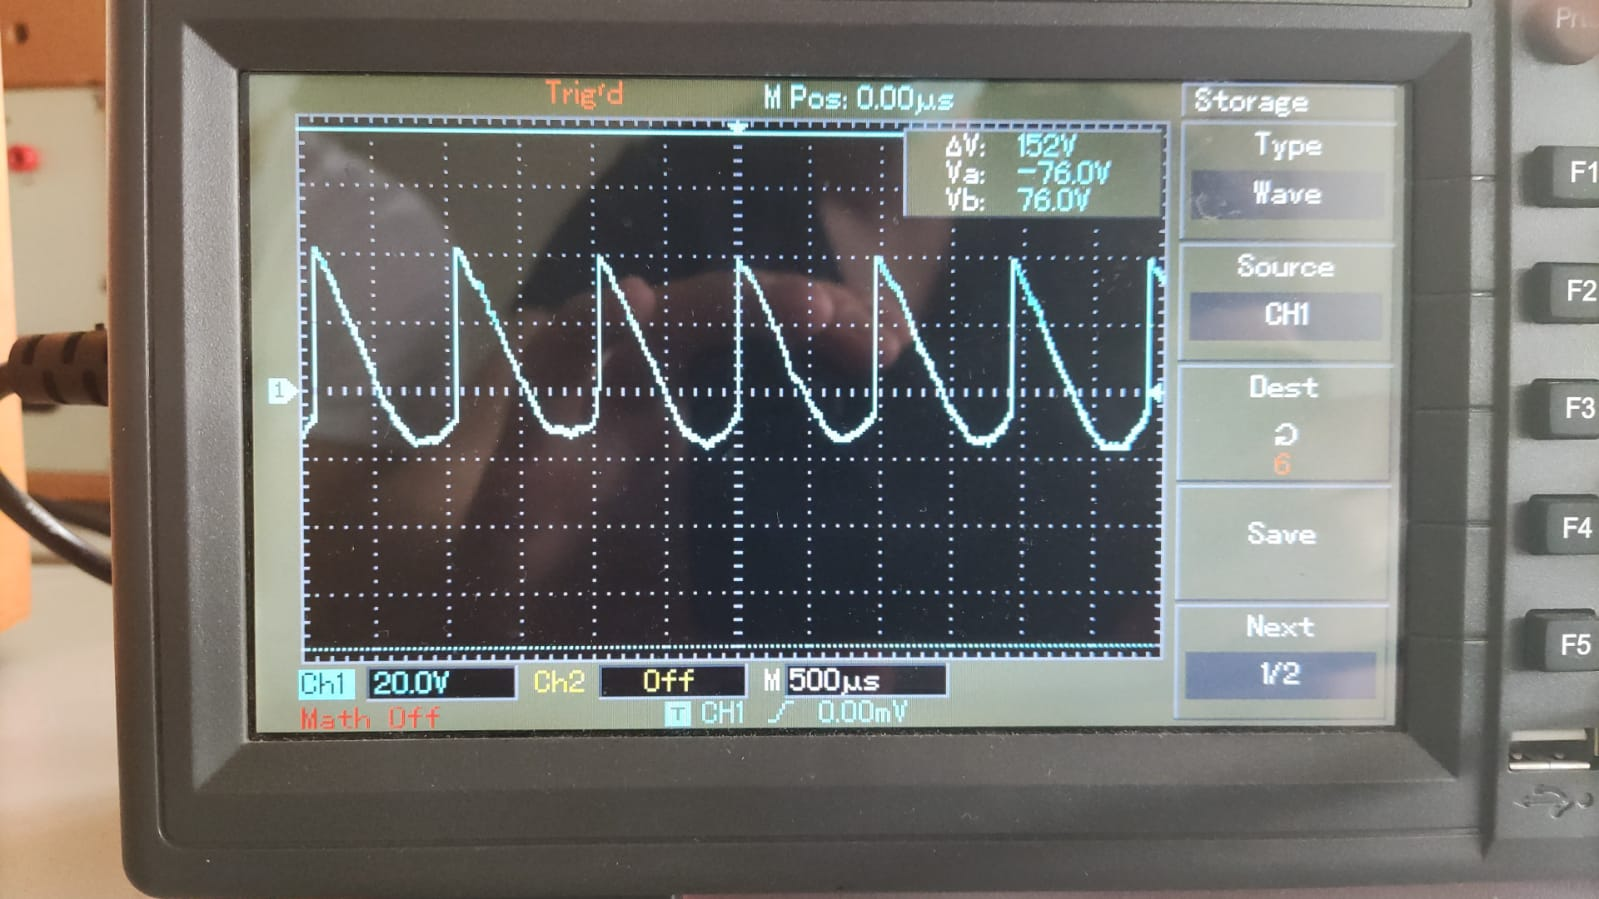
\includegraphics[height = 3.5cm]{data_scripts/pics/120m.jpeg}
            \caption{Mit Rauschen}
    \end{subfigure}
    \caption{Ausgangsspannung bei $\phi = \ang{120;;}$}
\end{figure}
\begin{figure}
    \begin{subfigure}{0.48 \textwidth}
        \centering
        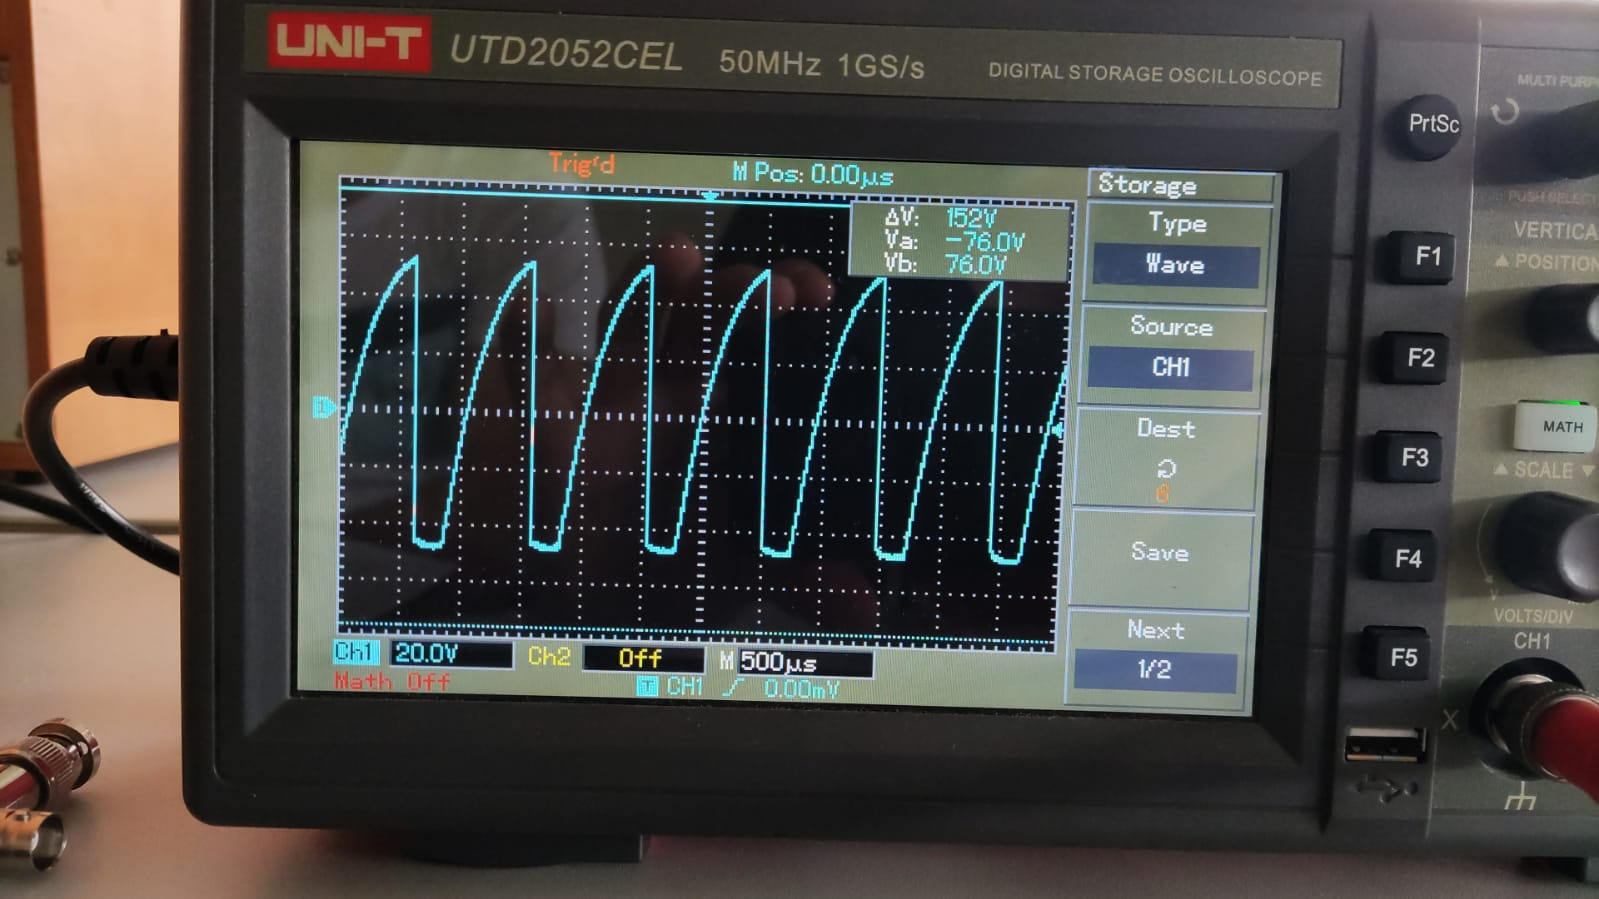
\includegraphics[height = 3.5cm]{data_scripts/pics/150o.jpeg}
        \caption{Ohne Rauschen}
    \end{subfigure}
    \hfill
    \begin{subfigure}{0.48 \textwidth}
            \centering
            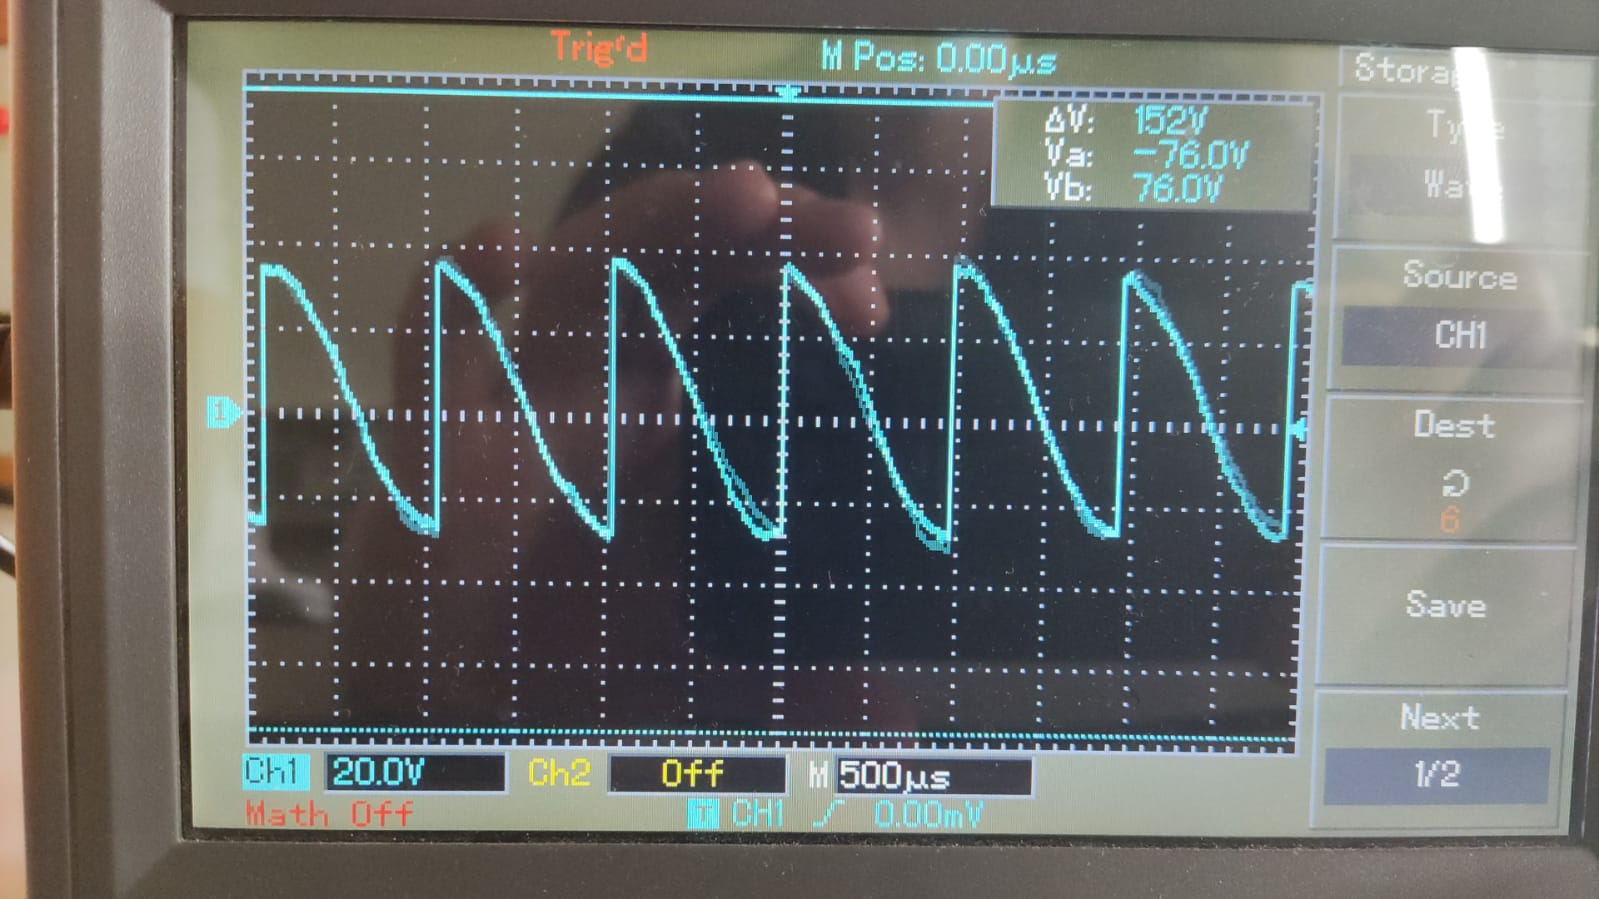
\includegraphics[height = 3.5cm]{data_scripts/pics/150m.jpeg}
            \caption{Mit Rauschen}
    \end{subfigure}
    \caption{Ausgangsspannung bei $\phi = \ang{150;;}$}
\end{figure}
\begin{figure}
    \begin{subfigure}{0.48 \textwidth}
        \centering
        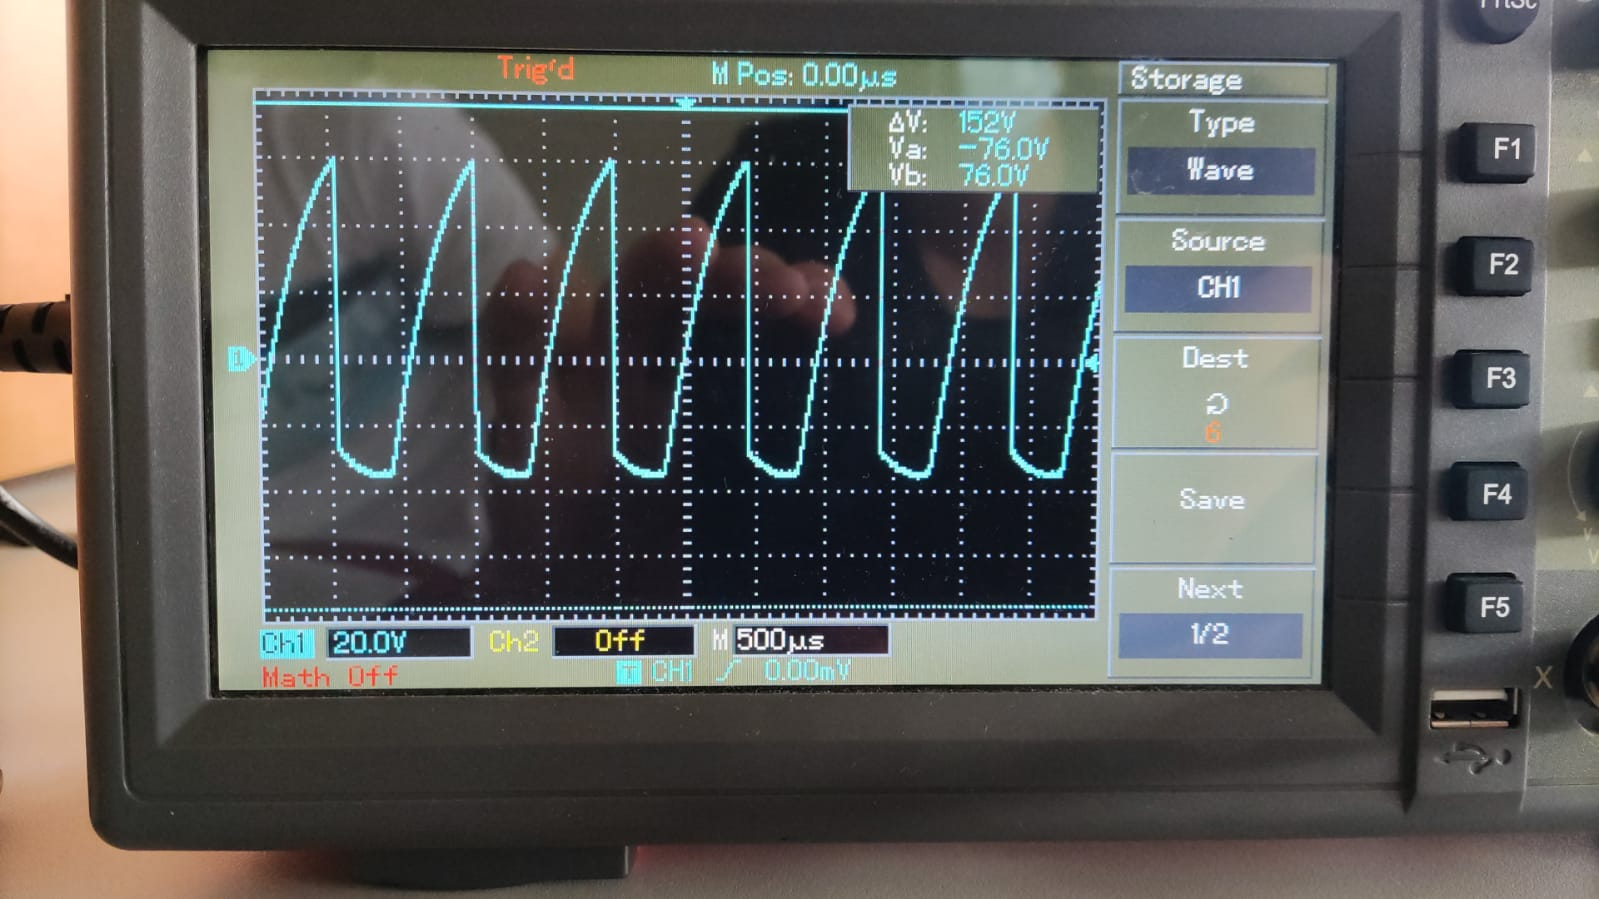
\includegraphics[height = 3.5cm]{data_scripts/pics/180o.jpeg}
        \caption{Ohne Rauschen}
    \end{subfigure}
    \hfill
    \begin{subfigure}{0.48 \textwidth}
            \centering
            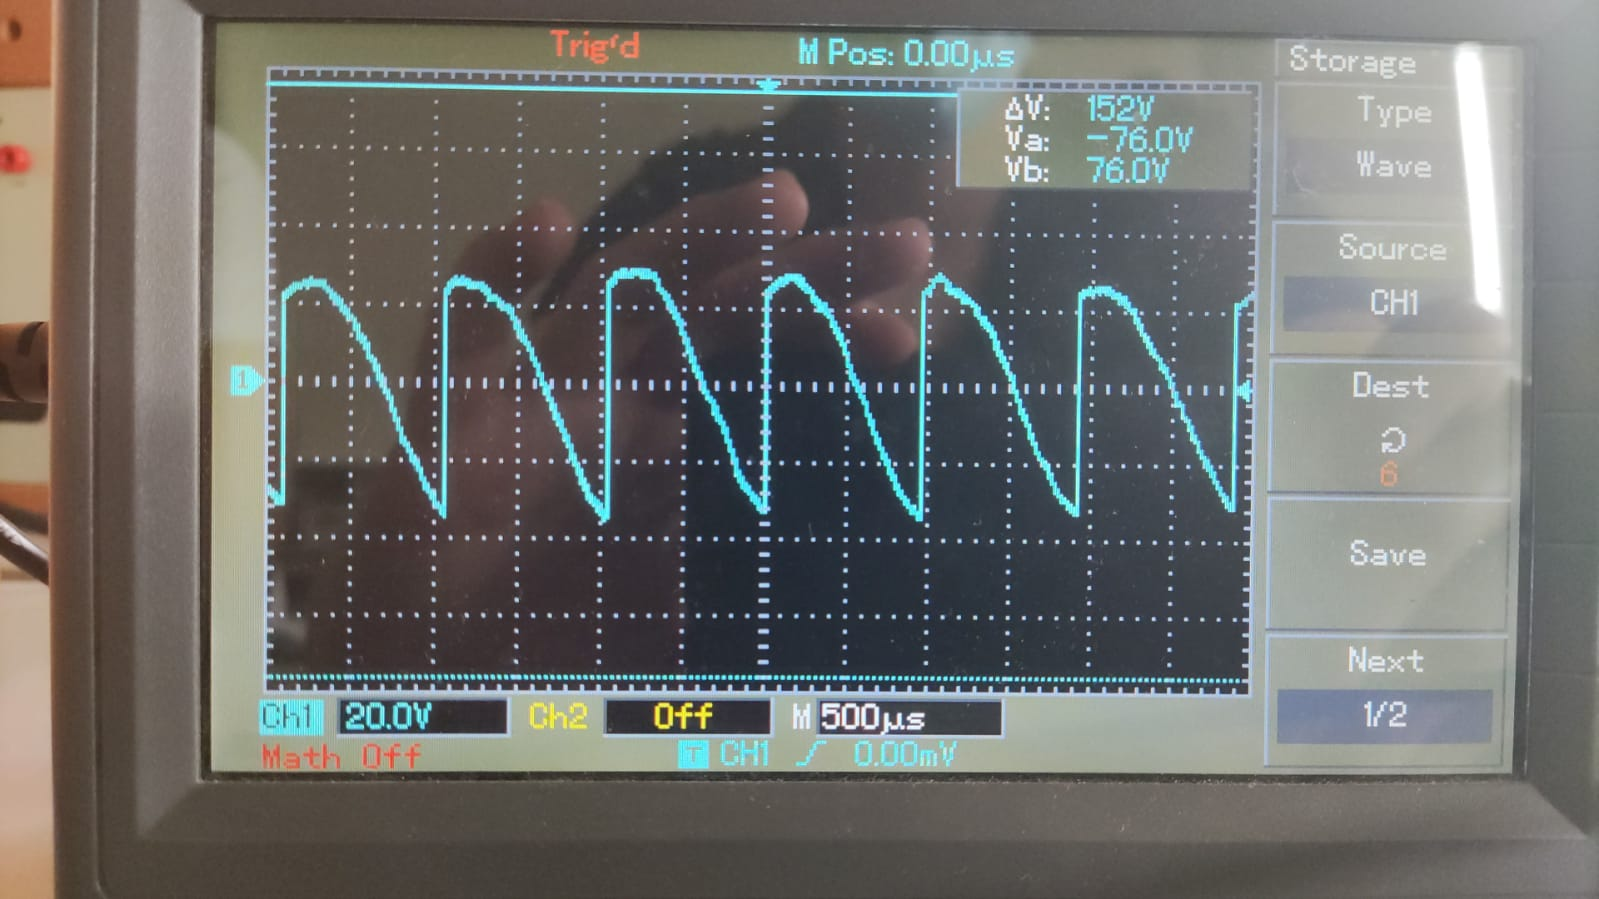
\includegraphics[height = 3.5cm]{data_scripts/pics/180m.jpeg}
            \caption{Mit Rauschen}
    \end{subfigure}
    \caption{Ausgangsspannung bei $\phi = \ang{180;;}$}
\end{figure}
In der Tabelle \ref{tab:voltage} sind die gemessenen Ausgangsspannungen in Abhängigkit von der Phase
$\phi$ aufgezeichnet. 
Dabei ist $U_\text{out}$ die unverrauschte Spannung und $U_\text{out}$ die verrauschte Spannung.
\begin{table}
    \centering
    \caption{Gemessen Ausgangsspannungen $U_\text{out}$ und $U_\text{out, noise}$}
    \label{tab:voltage}
    \begin{tabular} {S[table-format=3.0] S[table-format=3.0] S[table-format=3.0]}
        \toprule
        {$\phi \mathbin{/} \si{\degree}$} & {$U_\text{out} \mathbin{/} \si{\milli\volt}$} & {$U_\text{out, noise} \mathbin{/} \si{\milli\volt}$}\\
    \midrule
    0       & 96 & 96\\
    30      & 86 & 86\\
    60      & 58 & 33\\
    90      & 74 & 44\\
    120     & 110 & 110\\
    150     & 100 & 100\\
    180     & 96 & 96\\    
    \bottomrule
\end{tabular}
\end{table}
Aus der Tabelle \ref{tab:voltage} ergibt sich einerseits die Abbildung \ref{fig:Uwo} mit den unverrauschten 
Spannungen, anderseits die Tabelle \ref{fig:Uwi} mit den verrauschten Sapnnungen.
Dort sind die gemessenen Spannungen gegen die Phase aufgetragen.
Zusätzlich ist dort eine Ausgleichskurve gemäß der Beziehung \eqref{eqn:cosine} eingezeichnet, welche sich mittels 
\begin{equation}
    U_\text{out} = a\cos \left ( b \, \phi + c \right ) + d
\end{equation}
beschreiben lässt, wobei der Parameter $a$ die Amplitude $U_0$ ist.
Für die unverrauschte Spannung ergeben sich die Parameter zu    
\begin{align*}
    a &= \num{22.09(594)}       \\
    b &= \num{2.17(22)}         \\
    c &= \num{113.93(44)}       \\
    d &= \num{86.58(413)} \; \text{.}
\end{align*}
Die Regressionsparameter der verrauschten Messwerte werden zu
\begin{align*}
    a_\text{noise} &= \num{0.68(13)} \\           
    b_\text{noise} &= \num{2.11(19)}  \\            
    c_\text{noise} &= \num{113.64(35)}\\
    d_\text{noise} &= \num{2.54(9)}
\end{align*}
berechnet.
\begin{figure}
    \centering
    \caption{Gemessene Spannungen $U_\text{out}$ mit Regressionskurve}
    \label{fig:Uwo}
    \includegraphics{build/Uwo.pdf}
\end{figure}
\begin{figure}
    \centering
    \caption{Gemessene Spannungen $U_\text{out, noise}$ mit Regressionskurve}
    \label{fig:Uwi}
    \includegraphics{build/Uwi.pdf}
\end{figure}
Somit können die Spannungsaplituden $U_0$ gemäß
\begin{equation*}
    U_0 = \frac{\pi}{2} a
\end{equation*}
zu 
\begin{align*}
    U_0                 & = \SI{33.7}{\milli\volt} \\
    U_{0 \text{, noise}}& = \SI{1.07}{\milli\volt}
\end{align*}
bestimmt werden.
\FloatBarrier
\subsection{Überprüfung der Rauschunterdückung des Lock-In-Verstärkers mit einer Photodetektorschaltung}
In der Tabelle \ref{tab:distance} ist die gemessene Sapnnung $U$ in Abhängigkeit des Abstands $r$
zwischen der LED und der Photodiode aufgelistet.
Dazu sind die Messwerte inklusive Regressionskurven mit einer $\sfrac{1}{r}$- und 
$\sfrac{1}{r²}$ -Abhängigkeit in der Abbildung \ref{fig:distance} aufgetragen.
Die Regressionskurven haben die Form
\begin{equation*}
    U = \frac{a_1}{r} + b_1
\end{equation*}
und
\begin{equation*}
    U = \frac{a_2}{r²} + b_2 \; \text{.}
\end{equation*}
Dabei ergeben sich die Parameter zu
\begin{align*}
    a_1 &= \num{10.23(18)} \\
    b_1 &= \num{0.44(5)}    \\
    a_2 &= \num{41.72(28)}  \\
    b_2 &= \num{3.78(6)}    \; \text{.}
\end{align*}
\begin{table}
    \centering
    \caption{Gemessene Spannungen $U$ und in Abhängigkeit des Abstands}
    \label{tab:distance}
    \begin{tabular} {S[table-format=2.1] S[table-format=1.2 ]}
        \toprule
        {$r \mathbin{/} \si{\centi\metre}$} & {$U \mathbin{/} \si{\volt}$}\\
    \midrule
    4.7  &1.90 \\
    5.0  &1.70 \\
    6.0  &1.50 \\
    7.0  &1.40 \\
    8.0  &1.30 \\
    9.0  &1.15 \\
    10.0 & 1.00\\
    11.0 & 0.85\\
    12.0 & 0.70\\
    13.0 & 0.60\\
    14.0 & 0.50\\
    15.0 & 0.45\\
    16.0 & 0.40\\
    17.0 & 0.35\\
    18.0 & 0.30\\
    19.0 & 0.30\\
    20.0 & 0.25\\
    21.0 & 0.23\\
    28.0 & 0.10\\
    50.0 & 0.05\\
    80.0 & 0.04\\  
    \bottomrule
\end{tabular}
\end{table}
\begin{figure}
    \caption{Gemessene Spannungen und Regressionskurven in Abhängigkeit des Abstands}
    \label{fig:distance}
    \includegraphics{build/distance.pdf}
\end{figure}